\documentclass[aspectratio=169]{beamer}
\usepackage{listings}
\usepackage{tikz}
\usetikzlibrary{shapes,shapes.multipart,arrows,positioning}

\beamertemplatenavigationsymbolsempty

\lstset{
  basicstyle=\ttfamily,
}

\newcommand{\filename}[1]{\texttt{#1}}
\newcommand{\dirname}[1]{\texttt{#1/}}
\newcommand{\command}[1]{\texttt{#1}}
\newcommand{\variable}[1]{\textit{#1}}
\newcommand{\branchname}[1]{\texttt{#1}}

\title{Schema Inference on Wikidata}
\subtitle{Final presentation}
\author{Lucas Werkmeister}
\date{2019-02-20}

\begin{document}

\frame{\titlepage}

\begin{frame}
  \frametitle{Wikidata}
  \begin{figure}
    \includegraphics[width=0.7\textwidth]{item}
  \end{figure}
\end{frame}

\begin{frame}
  \frametitle{Wikidata}
  \begin{figure}
    \includegraphics[width=0.8\textwidth]{constraint}
  \end{figure}
\end{frame}

\begin{frame}[fragile]
  \frametitle{RDF}
  \begin{figure}
    \begin{lstlisting}[language=sparql]
wd:Q57385555 rdfs:label "Schema Inference on Wikidata"@en;
  schema:description "master thesis (2018) ..."@en;
  wdt:P31 wd:Q1907875; # instance of: master's thesis
  wdt:P1476 "Schema Inference on Wikidata"@en; # title
  wdt:P50 wd:Q57387675. # author: Lucas Werkmeister

wd:Q57387675 rdfs:label "Lucas Werkmeister"@en;
  wdt:P31 wd:Q5. # instance of: human
    \end{lstlisting}
  \end{figure}
\end{frame}

\begin{frame}[fragile]
  \frametitle{Shape Expressions (ShEx)}
  \begin{figure}
    \begin{lstlisting}[language=sparql]
<master_thesis> {
  wdt:P1476 xsd:langString; # title
  wdt:P50 @<human>+ # author
}

<human> {
  wdt:P569 xsd:dateTime; # date of birth
  wdt:P570 xsd:dateTime? # date of death
}
    \end{lstlisting}
  \end{figure}
\end{frame}

\begin{frame}
  \frametitle{RDF2Graph}
  \vspace{-5cm}
  \begin{figure}
    \centering
    % TODO horizontal zig-zag instead of 50% scale?
    \begin{tikzpicture}[transform canvas={scale=0.5}]
      \tikzstyle{file} = [rectangle, draw, rounded corners, text centered]
      \tikzstyle{pipe} = [style=file, dashed]
      \tikzstyle{directory} = [rectangle, draw, text centered]
      \tikzstyle{arrow} = [draw, -latex', right]

      \begin{scope}[node distance=2cm]
        \node[file] (entities) {\filename{\variable{example}.entities.sparql}};
        \node[file, below of=entities] (data) {\filename{\variable{example}.data.sparql}};
        \node[pipe, below of=data] (JSON) {\filename{\variable{example}.json}};
        \node[file, below of=JSON] (N-Triples) {\filename{\variable{example}.nt}};
        \node[directory, below of=N-Triples] (Fuseki) [align=center] {\dirname{\variable{example}-fuseki} \\ \texttt{http://localhost:3030/\variable{example}/query}};
        \node[directory, below of=Fuseki] (RDF2Graph) {\dirname{\variable{example}-results}};
        \node[file, below of=RDF2Graph] (ShEx) {\filename{\variable{example}.shex}};
        \node[file, below of=ShEx] (HTML) {\filename{\variable{example}.html}};
      \end{scope}

      \begin{scope}[every path/.style=arrow, midway]
        \path (entities) -- node {\command{sed}} (data);
        \path (data) -- node {WDQS} (JSON);
        \path (JSON) -- node {\command{jq}} (N-Triples);
        \path (N-Triples) -- node {Fuseki} (Fuseki);
        \path (Fuseki) -- node {RDF2Graph} (RDF2Graph);
        \path [dashed] (RDF2Graph.north east) to [out=30,in=330,looseness=5] node {RDF2Graph, simplify} (RDF2Graph.south east);
        \path (RDF2Graph) -- node {ShEx exporter} (ShEx);
        \path (ShEx) -- node {\command{pygmentize}} (HTML);
      \end{scope}
    \end{tikzpicture}
  \end{figure}
\end{frame}

\end{document}
